\chapter{A MDP e o ciclo de vida do produto}

\section{Distinção de tipo e instância de um ativo}

	O modelo do RAMI4.0 apresenta um eixo de ciclo de vida generalizado, derivado da norma IEC 62890 \cite{adolphs2015rami}. A ideia do trás do eixo Ciclo de Vida e Cadeia de Valor é distinguir todos os ativos na I4.0 entre tipos e instâncias:
	
	\begin{itemize}
	  \item Tipo: Presente desde a concepção/conceitualização até os primeiros protótipos/testes. O ``tipo'' de um ativo é definido e propriedades e funcionalidades distintas são definidas e implementadas. Todos os artefatos de design (interno) são criados, como dados CAD, esquemas, software incorporado e associados ao tipo de ativo. Aumentando a capacidade de produção. As informações 'externas' associadas ao ativo são criadas, como folhas de dados técnicos, informações de marketing. O processo de venda é iniciado.
	  
	  \item Instância: São criadas/produzidas com base nas informações de um tipo de ativo. Informações específicas sobre produção, logística, qualificação e teste estão associadas às instâncias do ativo. Fase de uso pelo comprador das instâncias do ativo. Os dados de uso estão associados à instância do ativo e podem ser compartilhados com outros parceiros da cadeia de valor, como o fabricante da instância do ativo.
	  Também inclui: manutenção, re-design, otimização e desativação da instância do ativo. O histórico completo do ciclo de vida está associado ao ativo e pode ser arquivado / compartilhado para documentação.
	  
	\end{itemize}

	Esse relacionamento deve ser mantido ao longo da vida das instâncias do ativo. Por esse relacionamento, as atualizações nos tipos de ativos podem ser encaminhadas para as instâncias de ativos, automaticamente ou sob demanda \cite{bader2019aas}.
	
	Os relacionamentos entre tipos e instância são cíclicos e possibilitam a retroalimentação de informações. Para os ativos do produto, por exemplo, informações sobre o uso e manutenção de instâncias do produto armazenadas na MDP podem melhorar a fabricação de novos produtos, além de causar melhorias no projeto do próximo tipo de produto.
	
	Portanto, o fluxo de informações entre tipos e instâncias de um produto são essenciais para a melhoria do projeto do produto. A Figura \ref{fig:aas-lifecycle} ilustra como ocorre a instancialização (criação de uma instância a partir de um tipo) e o uso da MDP das instância para a criação de novas versões de um 'tipo'.
	
	\begin{figure}[H]
	  \centering
	  \caption{Ciclo de vida do produto.}
	  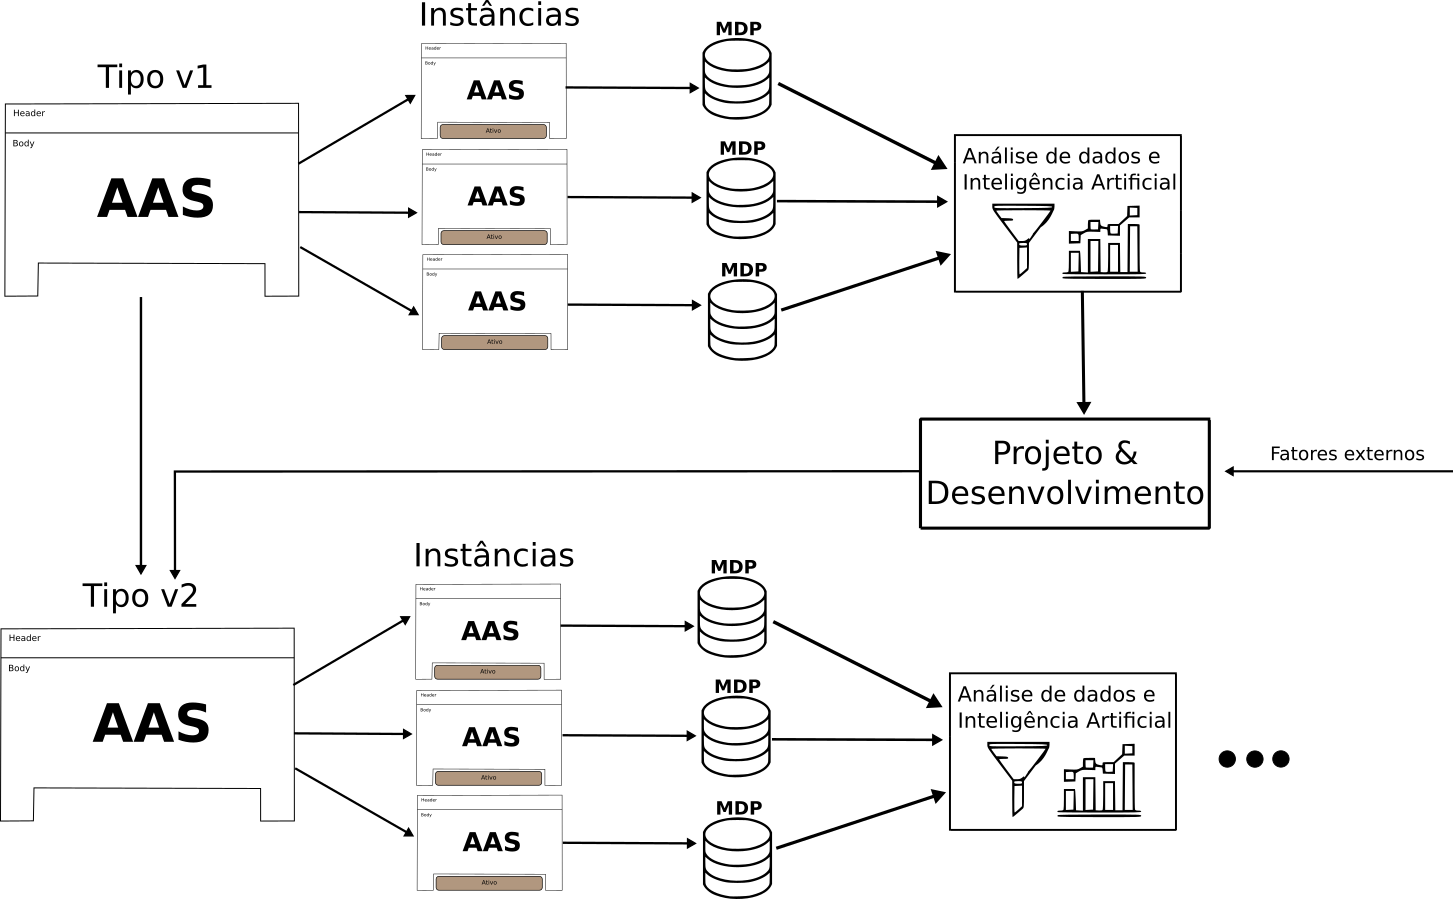
\includegraphics[width=1\textwidth]{aas-lifecycle.png}
	  \label{fig:aas-lifecycle}
	  \source{O autor.}
	\end{figure}


\section{Desenvolvimento do produto orientado a dados}

\lipsum[1-1]

\section{Manutenção do produto orientado a dados}

\lipsum[1-1]